\chapter{Datensätze}\label{cpt:datasets}
Diese Arbeit wie bereits in der Einführung erläutert, ist ein Aspekt dieser Arbeit den VAE basierten Data Augmentation Ansatz auf unterschiedlichen Daten zu evaluierten. Dazu werden sowohl Bilddaten, als auch numerische Daten evaluiert. Zusätzlich wird die Datensatzgröße variiert. Im folgenden werden die verwendeten Datensätze und ihre Besonderheiten näher beschrieben.



\section{MNIST}\label{sec:MNIST}
\begin{figure}[hbt]
  \centering
  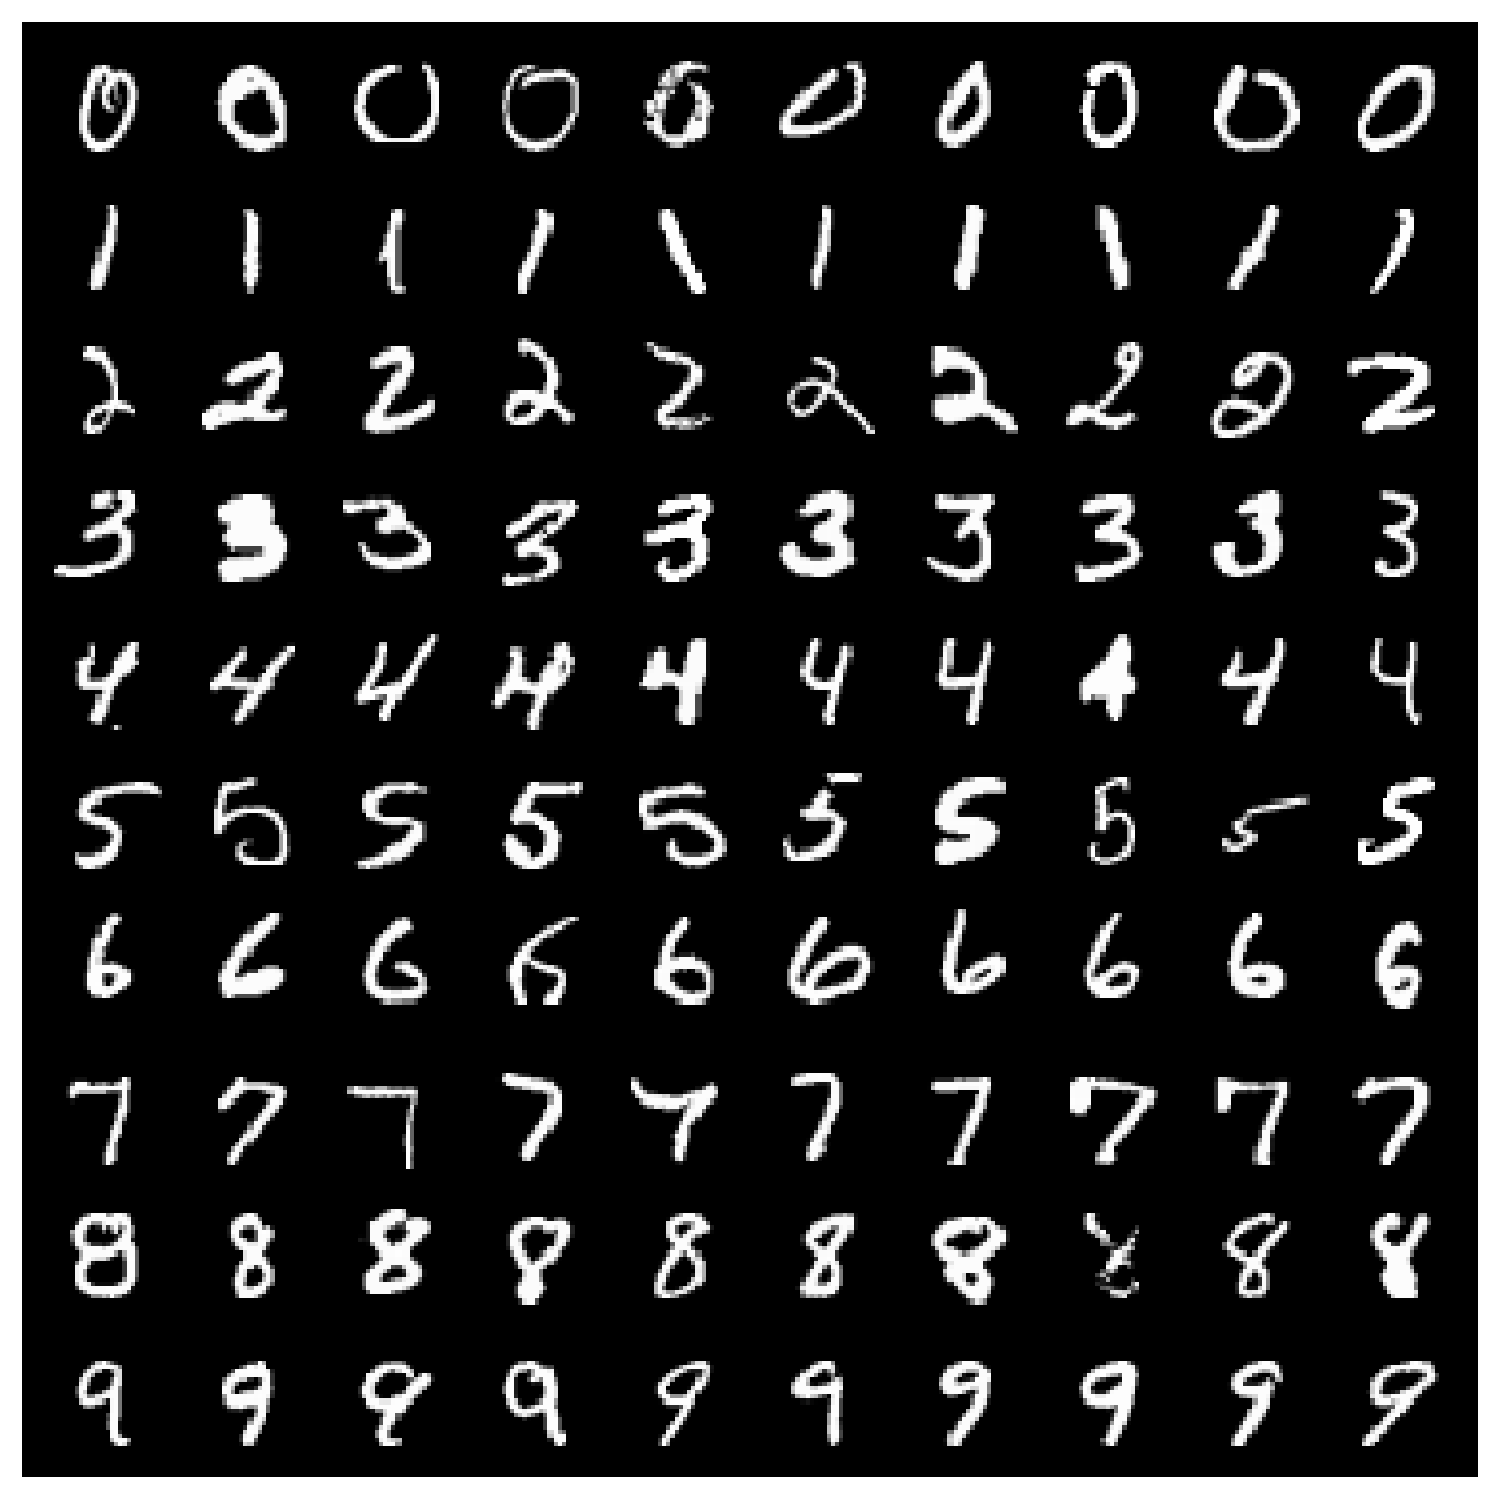
\includegraphics[width=.4\textwidth]{gfx/datasets/mnist_ciffers}
  \caption{Der MNIST Datensatz beinhaltet annotierte Bilder der handgeschriebenen Zahlen $\lbrace0, \dots, 9\rbrace$}
\end{figure}
Der MNIST Datensatz von \cite{lecun-98} wird oft verwendet, um neue Ansätze im Bereich Visual Machine Learning auf ihre Nutzbarkeit hin zu untersuchen. Es handelt sich bei den Daten um $(28 \times 28)$ Pixel große Grauwertbilder handgeschriebener Zahlen $\lbrace0, \dots, 9\rbrace$. Es gibt zwei Partitionen des Datensatzes: Die Trainings-Partition besteht aus 60.000 Beispielen, also 6.000 pro Klasse. Die Test-Partition beinhaltet 10.000 Beispiele. Die Klassifikation von MNIST ist über die letzten Jahre nahezu fehlerfrei gelöst (z.B. von \cite{byerly2021branching}), da die Daten klar voneinander unterscheidbar sind, der Datensatz balanciert ist und ausreichend Beispiele besitzt. \\

Da die MNIST Aufgabe wegen der genannten Eigenschaften schon durch einfache Modelle gut gelöst werden kann, werden in dieser Arbeit ausschließlich reduzierte Versionen des Originaldatensatzes betrachtet. Die Reduktion erfolgt durch zufälliges Wählen von Beispielen aus der Trainings-Partition des Datensatzes. Für die Evaluation wird der unveränderte Test-Teil verwendet.



\section{PROBEN1}\label{sec:PROBEN1_dataset}
PROBEN1 ist eine Zusammenfassung mehrerer Datensätze, welche verschiedenste Diagnoseinformationen (Attribute) enthalten, die eine Klassifikation ermöglichen. Vorgeschlagen wurde dieser Datensatz von \cite{Moreno-Barea2020} um verschiedene Generative Modelle auf kleinen teilweise imbalancierten Datensätzen zu evaluieren. Es ist ein rein numerischer Datensatz, bei dem jede Dimension des Eingabevektors ein Attribut (z.b. Alter, BMI, etc.) beschreibt. Nicht alle diese Attribute entsprechen kontinuierlichen Werten, daher wurden alle Daten, kontinuierliche und diskrete, normalisiert. Fehlende Daten (im Original durch ein "?" repräsentiert) wurden durch Nullen ersetzt. Im Gegensatz zu MNIST und anderen Bild-Datensätzen spielt die relative Position der Attribute im Eingabevektor keine Rolle. Dies wird bei der Wahl der Modellarchitektur für diesen Datensatz berücksichtigt.
 Tabelle \ref{tab:PROBEN1-datasets} gibt einen Überblick über die Dimension der Eingabevektoren (\# Attribute), die Anzahl an Klassen und die Größe und Balance der einzelnen Datensätze.
\begin{table}[hbt]
\centering
\begin{tabular}{l|l|l|l|l|l}
\toprule
Datensatz   & \# Attribute & kontinuierlich        & \# Klassen & \# Beispiele & Balancing \\ \hline
card        & 15           & 0.40                  & 2          & 690          & 0.99      \\
diabetes    & 8            & 1.00                  & 2          & 768          & 0.93      \\
geneN       & 60           & 0.00                  & 3          & 3175         & 0.93      \\
glass       & 9            & 1.00                  & 6          & 214          & 0.84      \\
horse-colic & 20           & 0.70                  & 3          & 364          & 0.84      \\
thyroid     & 21           & 0.29                  & 3          & 7200         & 0.28      \\
\bottomrule
\end{tabular}
\caption{PROBEN1 Datensatz Infos.}
\label{tab:PROBEN1-datasets}
\end{table}
Für diese Arbeit wurde jeder Datensatz in Trainings und Test-Partition aufgeteilt, wobei 80\% für das Training und 20\% für die Evaluation verwendet wurden. Zusätzlich werden reduzierte Trainings-Partitionen, analog zum Abschnitt \ref{sec:MNIST} betrachtet.


\section{CIFAR-10}
\begin{figure}[hbt]
  \centering
  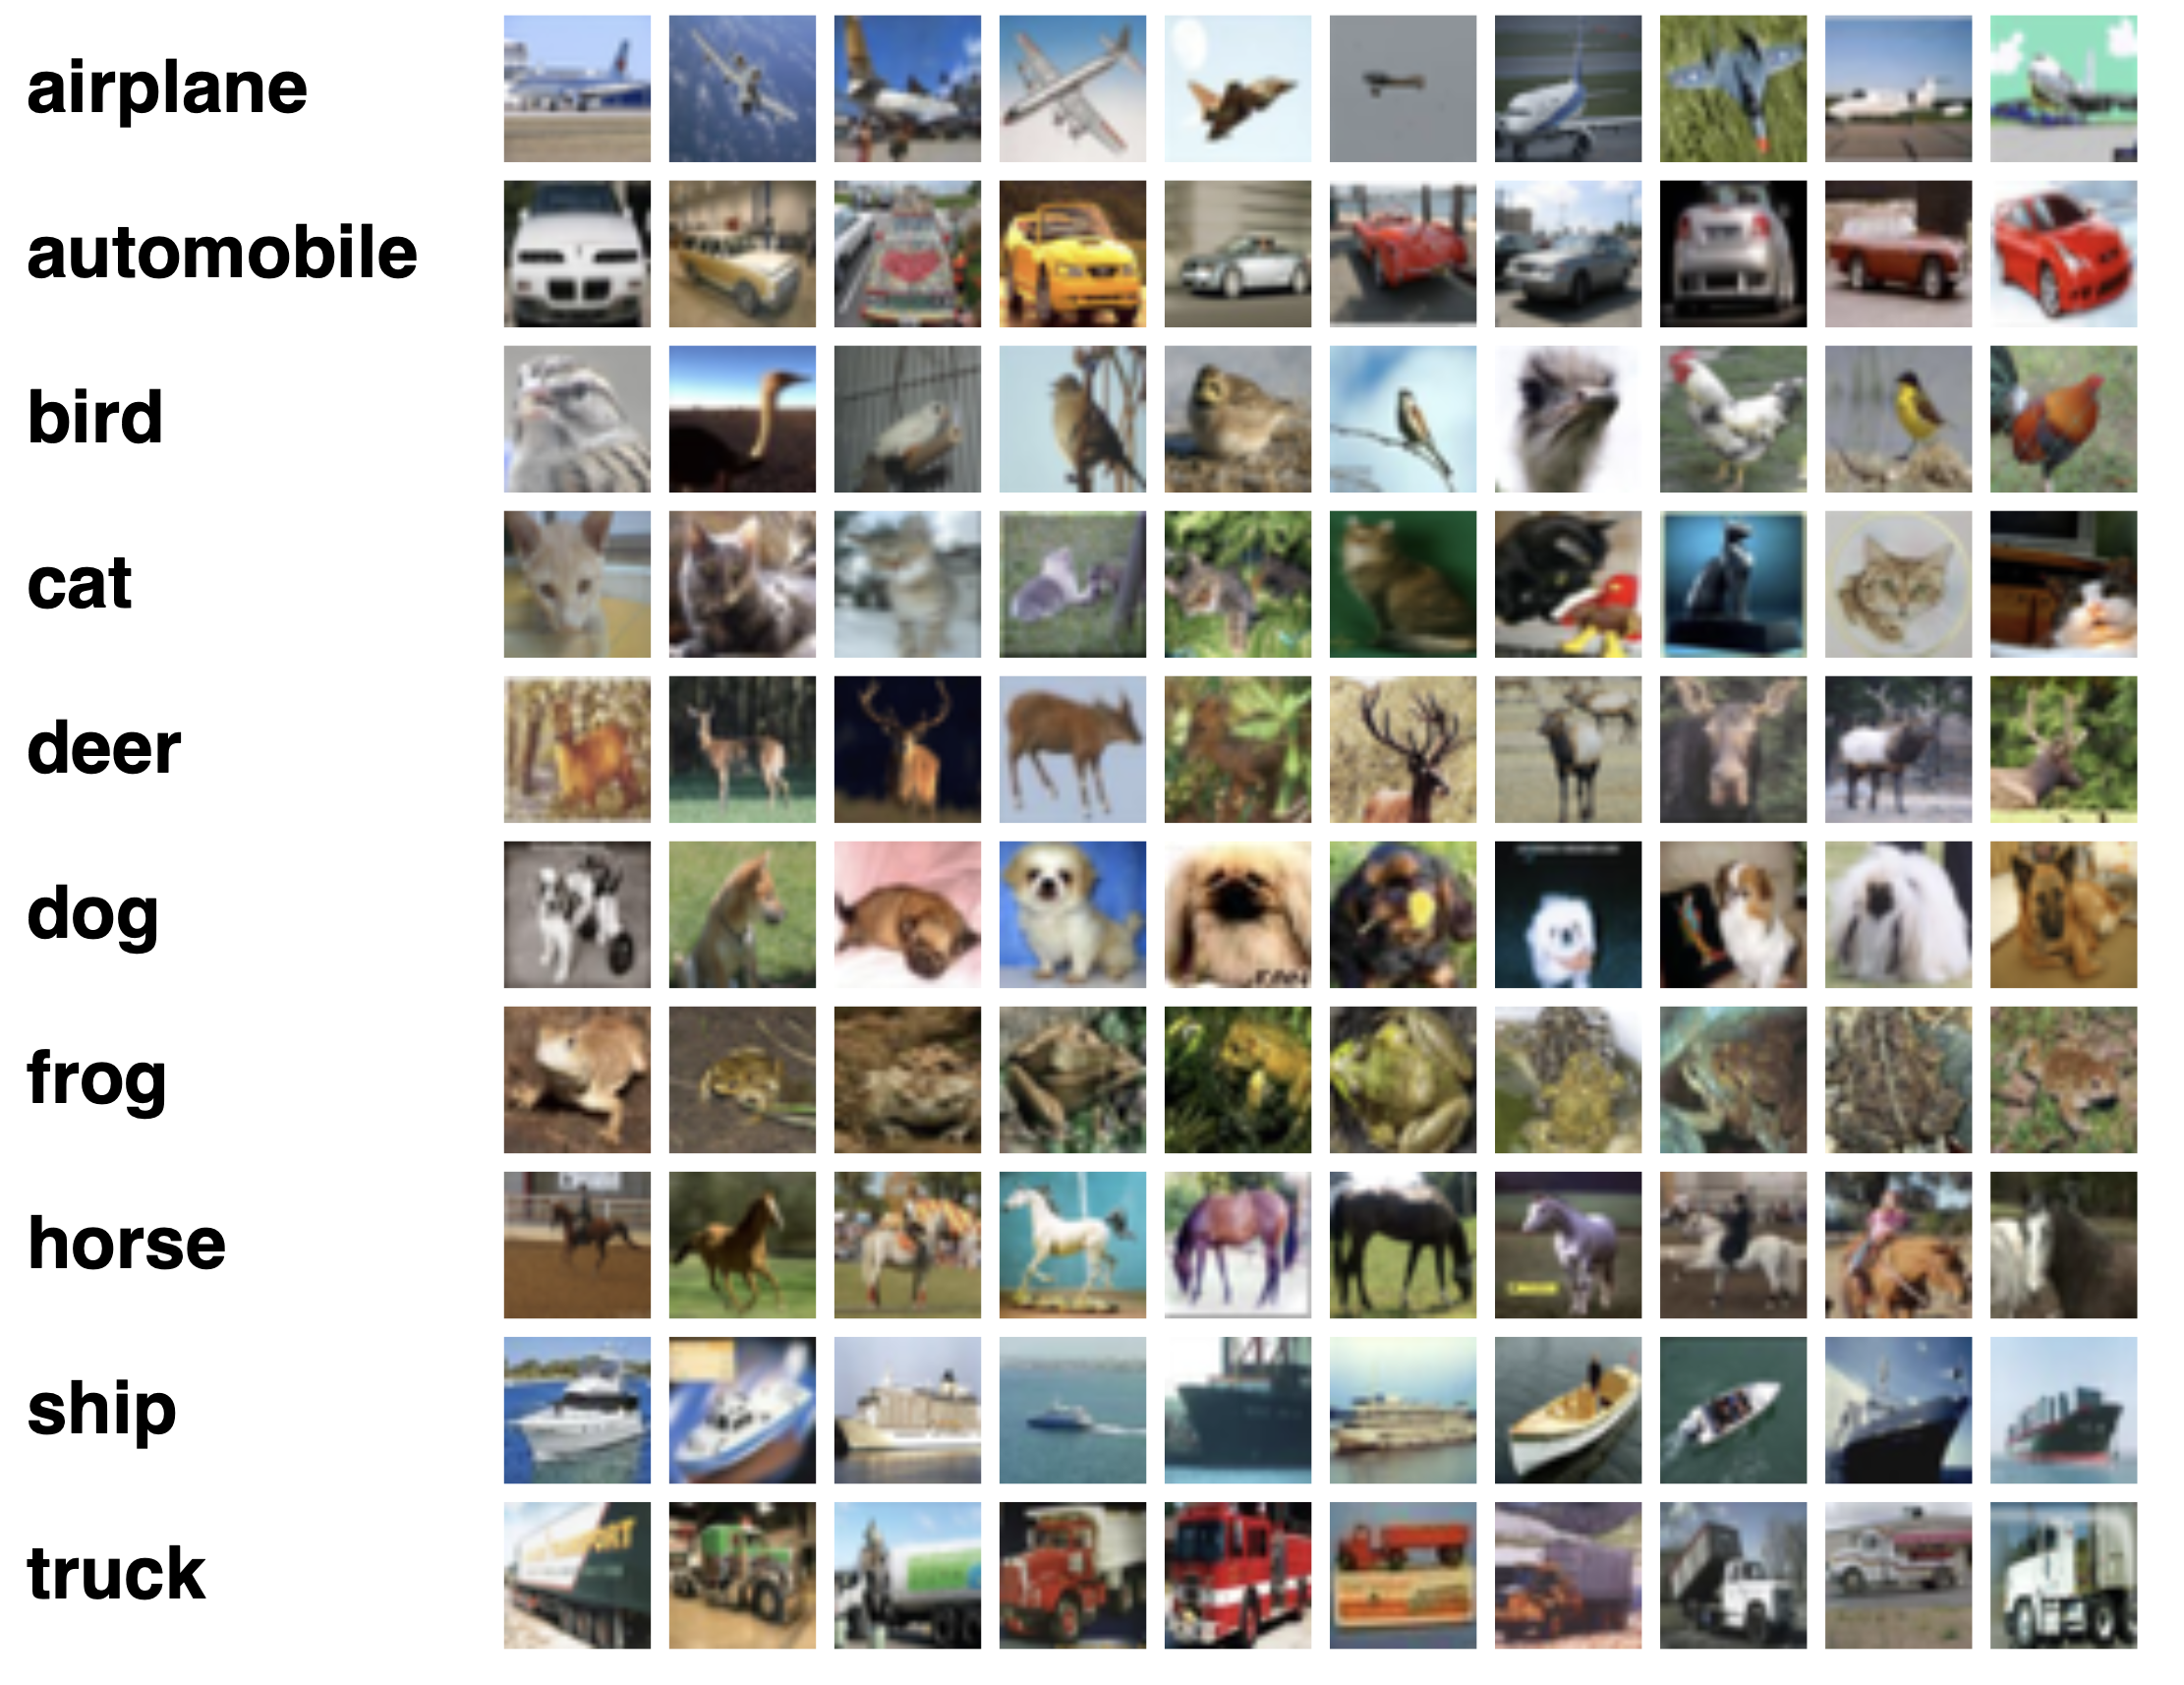
\includegraphics[width=.55\textwidth]{gfx/datasets/cifar10_dataset}
  \caption{CIFAR-10 Datensatz: Die einzelnen Klassen schließen sich gegenseitig aus, d.h. es gib z.b. keine Mischform aus "truck" und "automobile" wie SUV.}
  \label{fig:CIFAR_10_dataset}
\end{figure}
CIFAR-10 erstellt von \cite{cifar-orig} ist eine annotierte Teilmenge des "80 million tiny images" Datensatzes. Der Datensatz ist analog zu MNIST (vgl. Abschnitt \ref{sec:MNIST}) aufgeteilt in 60.000 Trainingsbeispiele und 10.000 Testbeispiele. Er enthält 10 verschiedene Klassen (siehe Abb. \ref{fig:CIFAR_10_dataset}). CIFAR-10 stellt als Klassifikationsaufgabe, wie MNIST, keine große Herausforderung da (siehe \cite{foret2021sharpnessaware}). Daher fokussiert sich diese Arbeit vor allem auf die Qualität der Rekonstruktionen auf diesem Datensatz.



\section{Large-scale CelebFaces Attributes}
\begin{figure}[hbt]
  \centering
  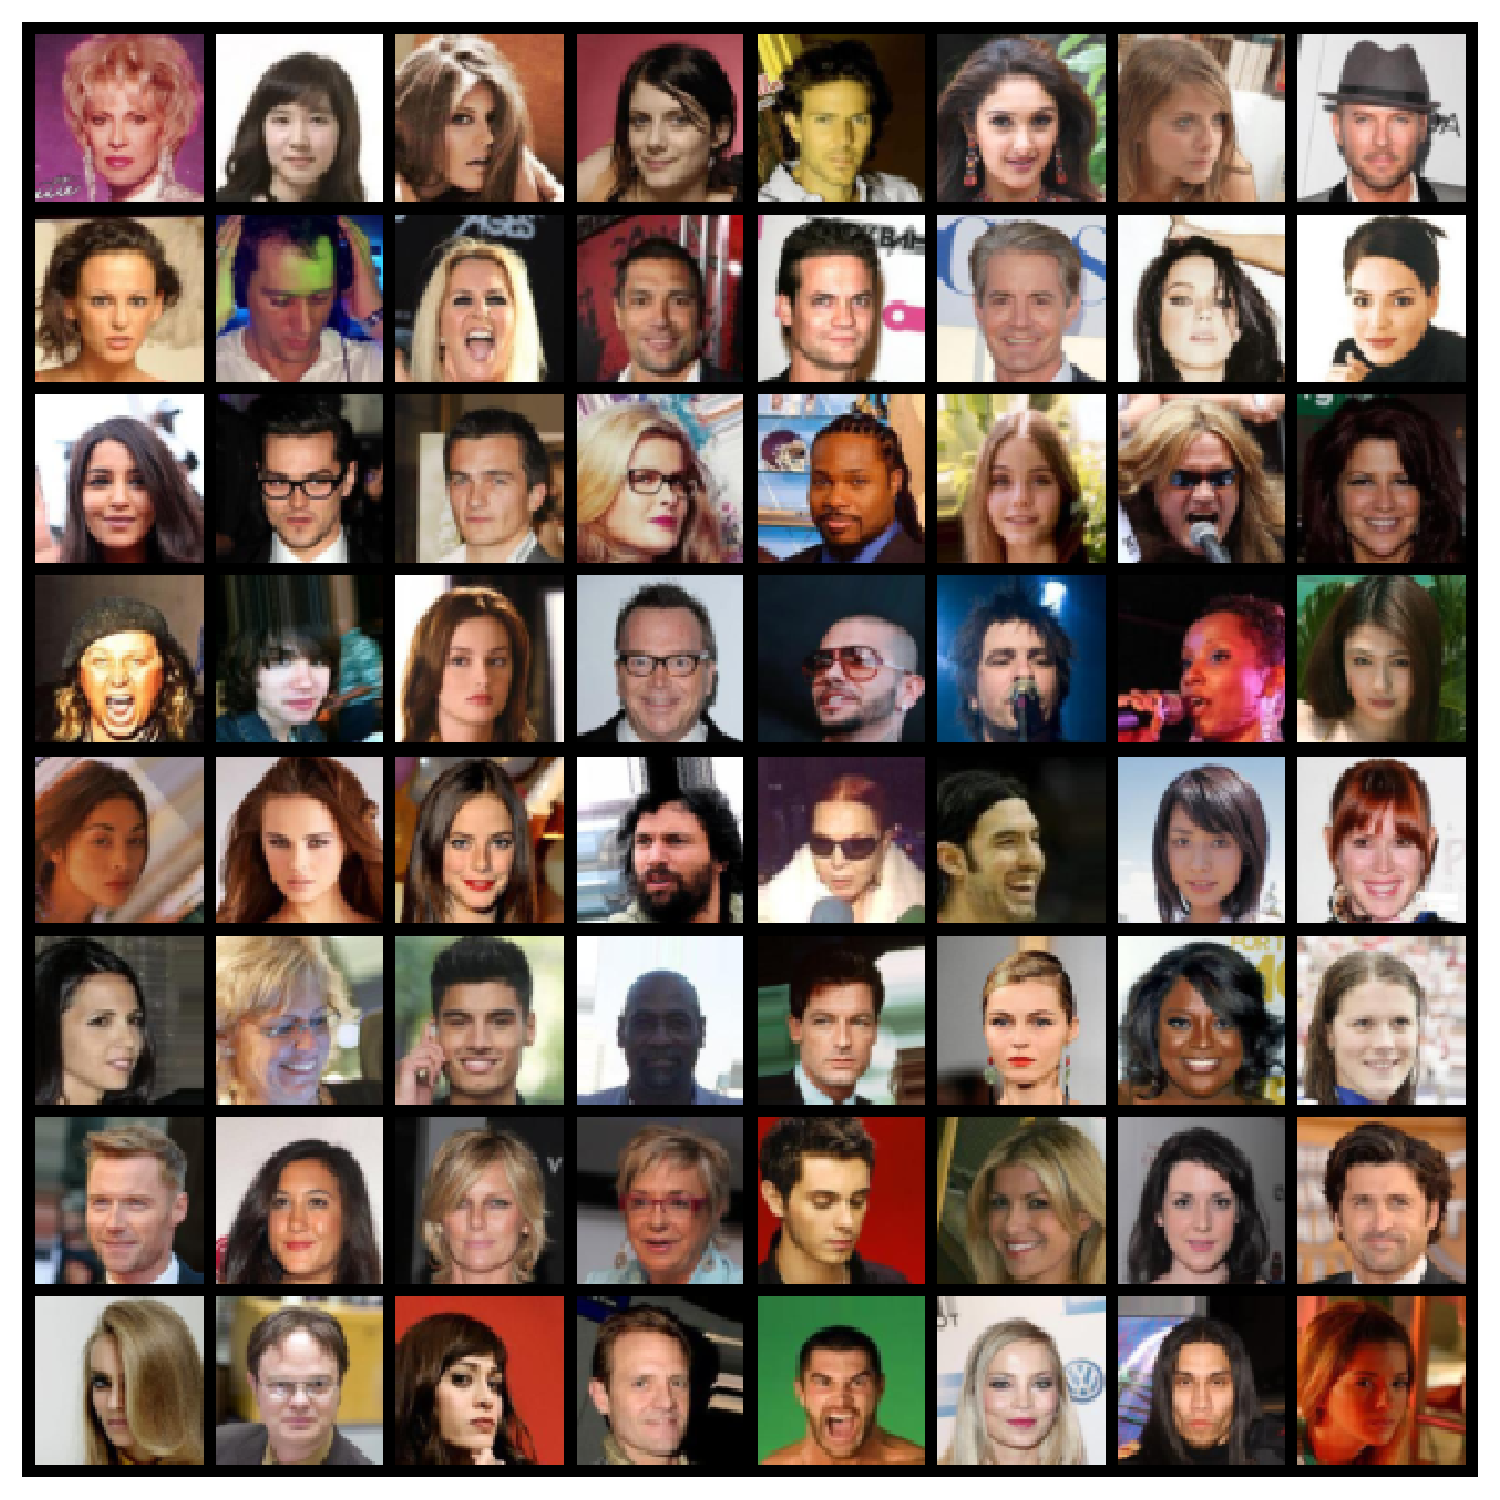
\includegraphics[width=.4\textwidth]{gfx/datasets/real}
  \caption{Die Gesichtsdaten des CelebA Datensatzes}
\end{figure}

Large-scale CelebFaces Attributes (CelebA), von \cite{liu2015faceattributes}, ist eine Sammlung von über 200.000 Bildern von Gesichten. Es gibt 10.177 verschiedene Identitäten. Jedes Bild ist mit 40 Attributen wie Haarfarbe, Brille, etc. annotiert. In dieser Arbeit wird insbesondere untersucht, wie sich Manipulationen im Merkmalsraum auf die decodierten Bilder auswirken. Da CelebA ein Multi-Label Datensatz ist (d.h. Attribute schließen sich gegenseitig nicht aus), liegt der Fokus auf der Trennung dieser Attribute im Latent-Space.
